\documentclass{article}
\usepackage[section]{placeins}
\usepackage{graphicx, wrapfig, amsmath, amssymb, physics, hyperref, mathtools}
\hypersetup{
    colorlinks=true,
    linkcolor=blue,
    filecolor=magenta,      
    urlcolor=cyan,
    }

\author{Yaghoub Shahmari}
\title{Report - Problem Set No 6}
\date{\today}
\graphicspath{ {../Figs/} }

\begin{document}
    \maketitle
    \section{RC circuit equation}
    \textbf{Basic description:}

    In an RC circuit, the amount of electric charge passing through the circuit is as follows:

    $$R \frac{d q}{d t}+\frac{q}{C}=V_0 \Rightarrow \dot{q} = \frac{V_0}{R} - \frac{q}{RC}  \xRightarrow[q_{(0)} = 0]{q_0 \coloneqq V C} q_{(t)}=q_0 (1-e^{-t/RC})$$

    where C, V, and R are the potential difference, capacitor capacity, and circuit resistance, respectively.
    
    I have solved this equation with RK1(Euler), RK2, and RK4 methods. Below you can see the results next to the exact answer:

    \textbf{The results:}

    \begin{figure}[!htb]
        \centering
        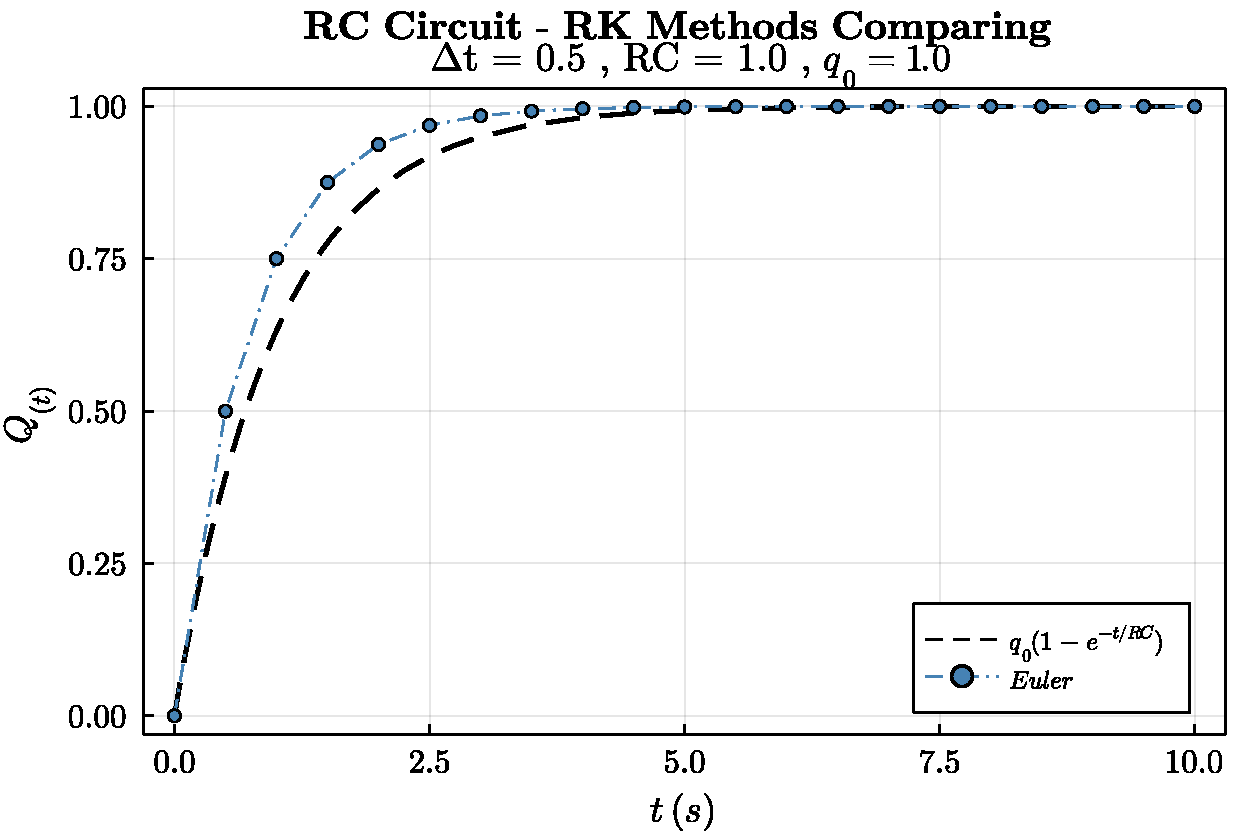
\includegraphics[scale = 0.25]{/Q1/RCEu}
        \label{fig:1.1}
        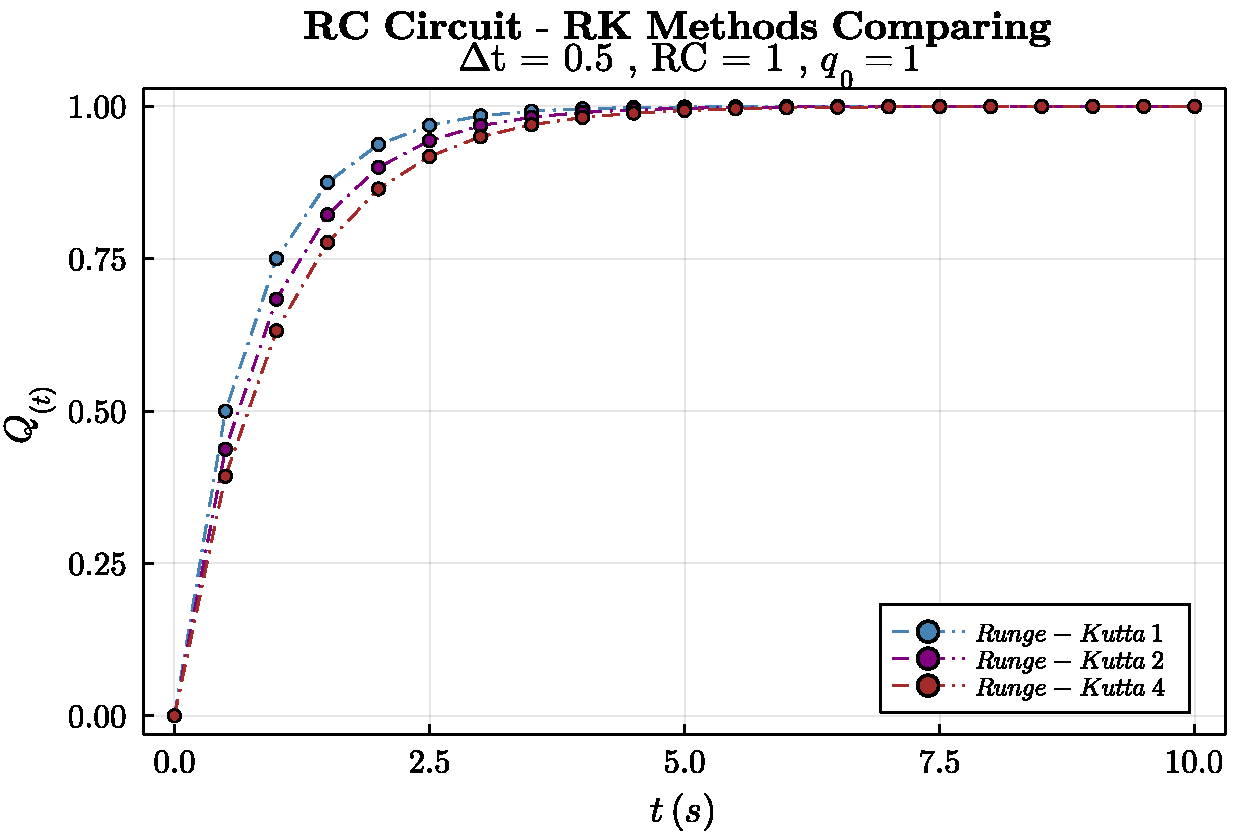
\includegraphics[scale = 0.25]{/Q1/RKComp}
        \label{fig:1.2}
        \caption{Plot of the results of the mentioned methods.}
    \end{figure}

    \pagebreak

    And at last, we want to find and analyze the effect of $\Delta t$ in the amount of global error for each method.
    We calculated the global error for a range of $\Delta t$ and drew the results in the following graph:

    \begin{figure}[!htb]
        \centering
        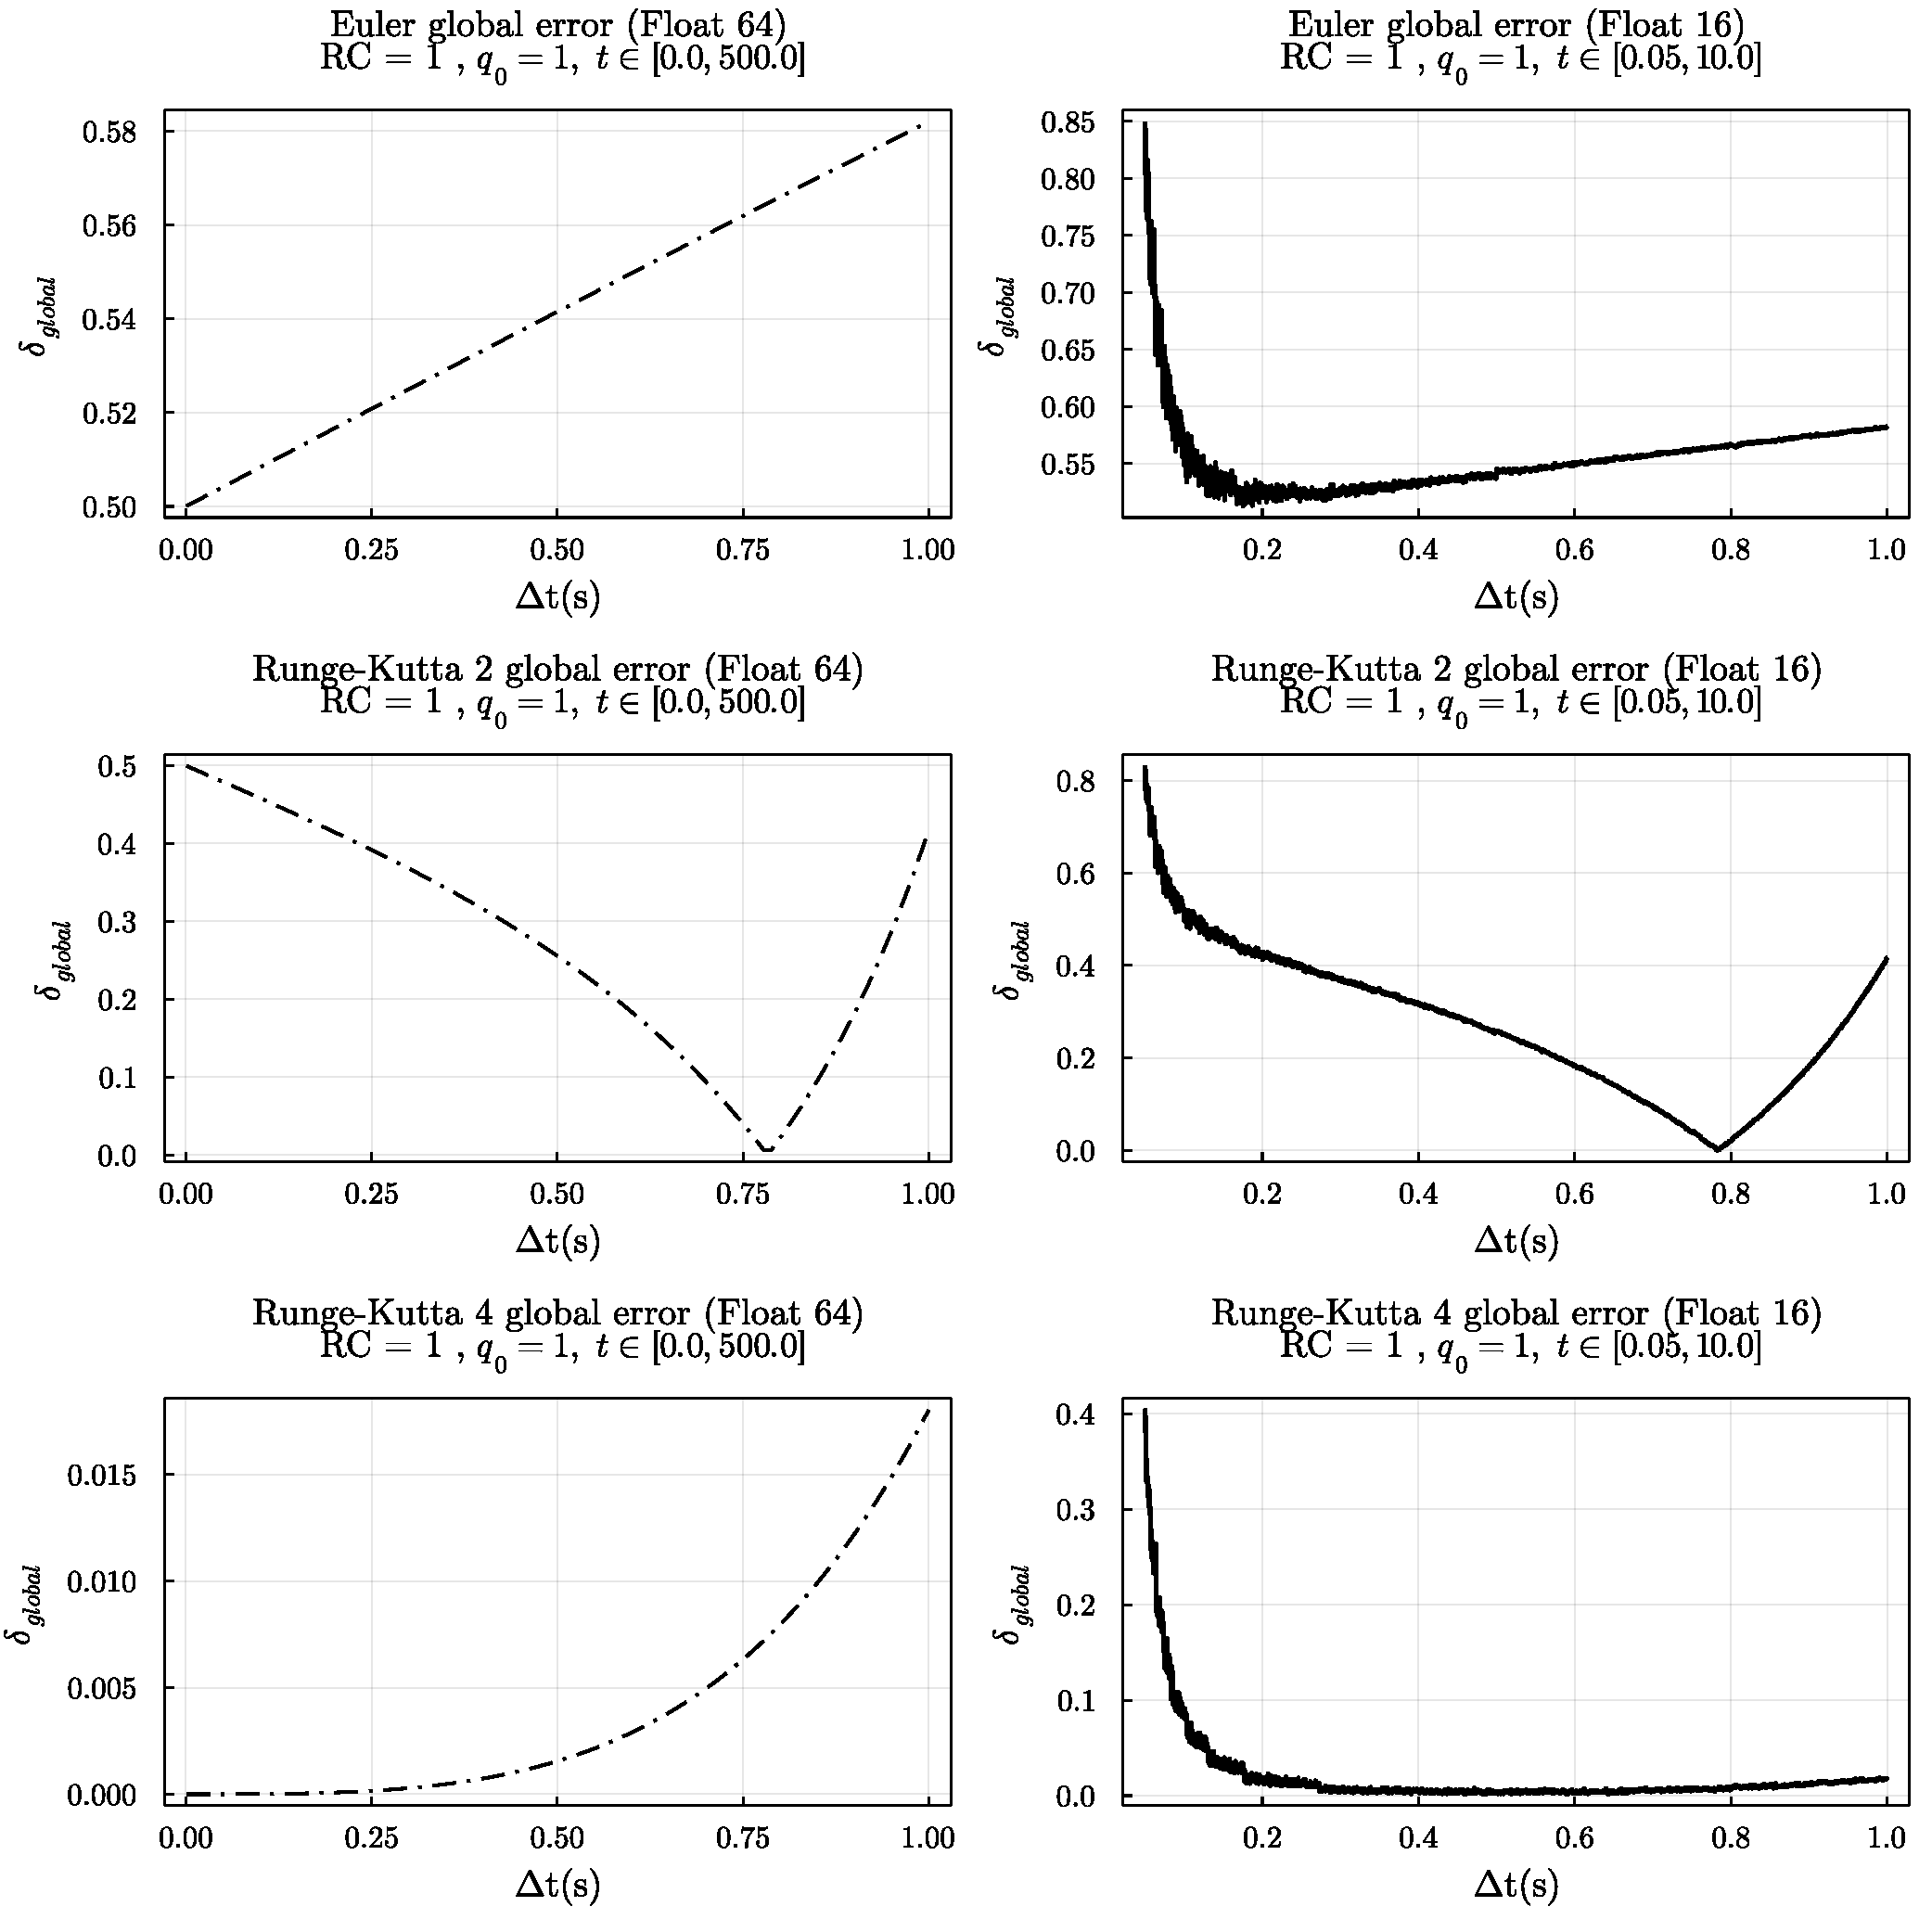
\includegraphics[scale = 0.3]{/Q1/error}
        \label{fig:1.3}
        \caption{Plot of the global error for each $\Delta t$.}
    \end{figure}

    To show the effect of floating-point error,
    I exported data in two types of float16 and float64.
    For float64 we can't find floating-point error well but in float16 type,
    it is easier to find the effect.

    As the final part of this section, we will solve the above equation with an unstable method presented in class. The results are as follow:

    \begin{figure}[!htb]
        \centering
        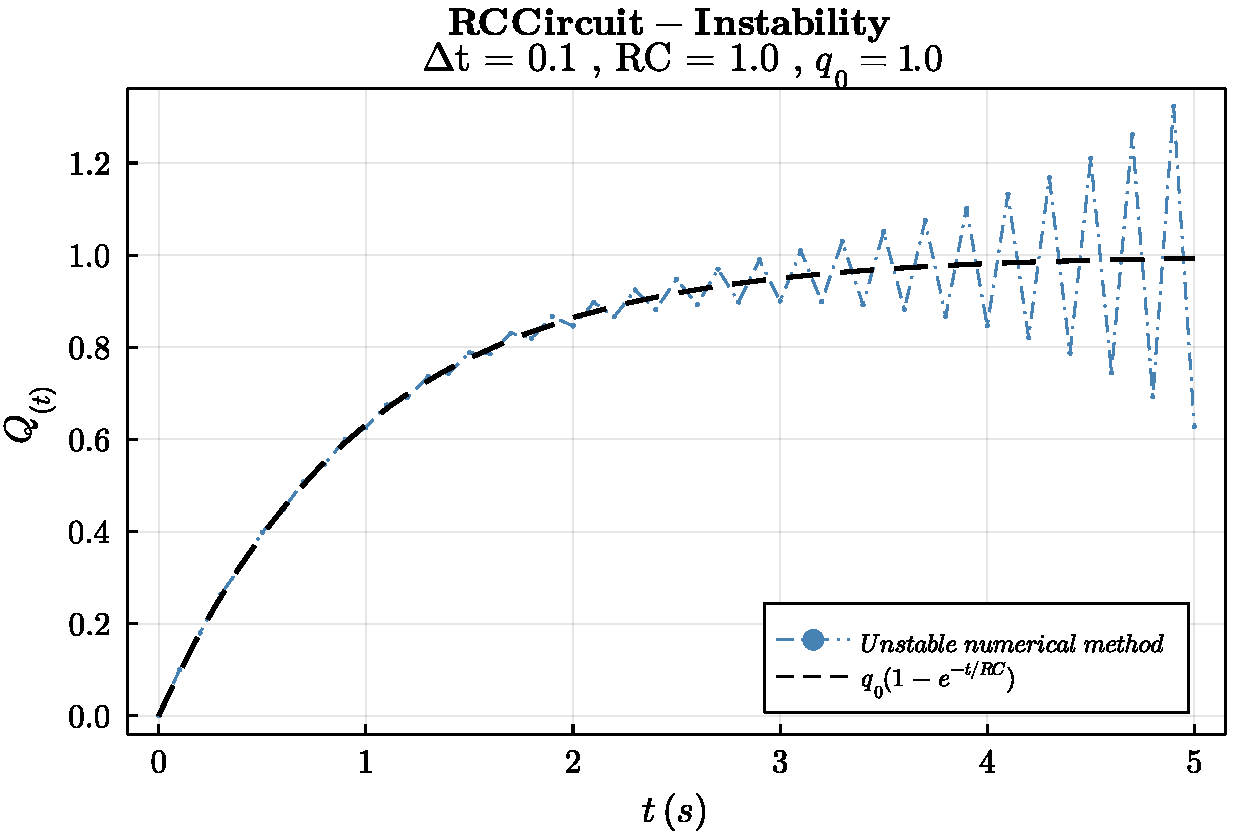
\includegraphics[scale = 0.5]{/Q1/Instability}
        \label{fig:1.4}
        \caption{Plot of the results of the mentioned method and the exact answer.}
    \end{figure}

    \section{Simple Harmonic Osillation}
    \textbf{Basic description:}
    
    In this section, we want to solve the second-order equation of simple harmonic oscillation using numerical methods.
    The oscillator follows this equation:

    $$
    \ddot{x} = -\omega x \Rightarrow
    \begin{cases}
        x(t) = x_0\cos(\omega t) \\
        v(t) = x_0\omega\sin(\omega t)
    \end{cases}
    $$

    which the $\omega$ is angular velocity and $x_0$ is the initial position.

    \begin{figure}[!htb]
        \centering
        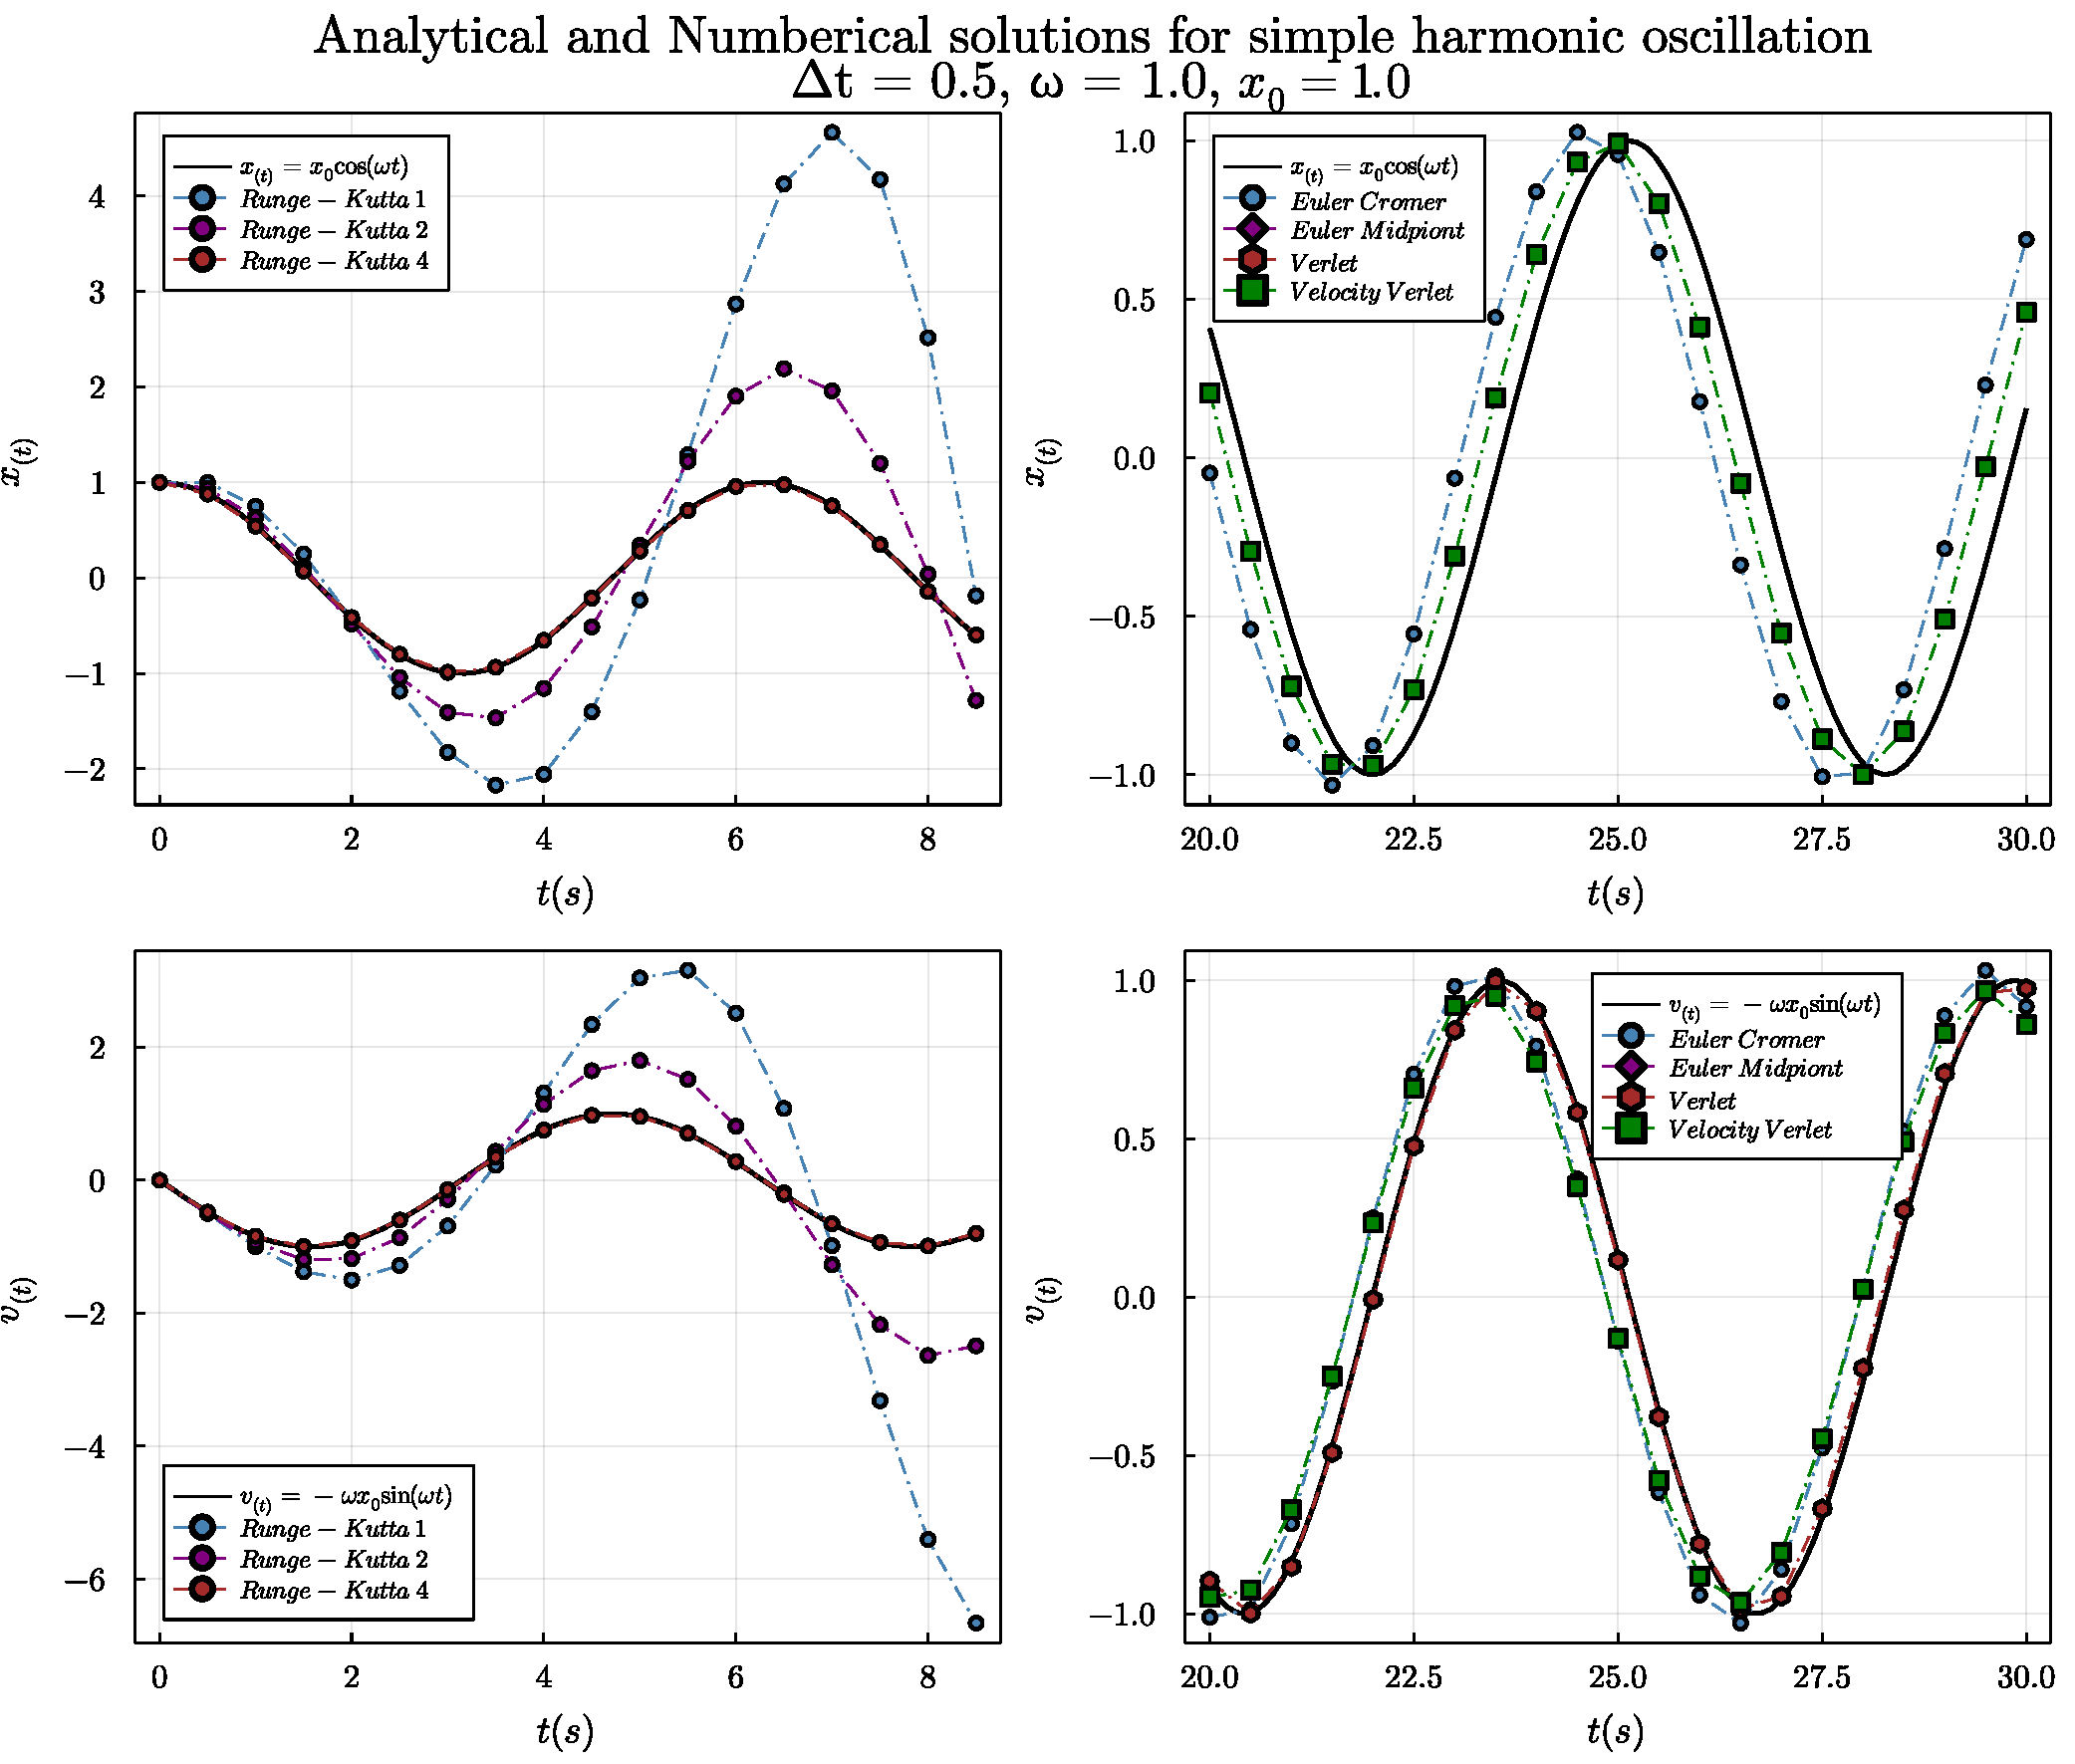
\includegraphics[scale = 0.3]{/Q2/SHO}
        \label{fig:2.1}
        \caption{Plot of the numerical solution for each method and the exact answer for simple harmonic oscillation.}
    \end{figure}

    As you can see, the RK4 method has the best accuracy among the other methods.
    Also, it is obvious that RK1 and RK2 methods are unstable and do not follow the energy conservation.

    As the final part of this section,
    we drew the phase diagram of oscillation.

    \begin{figure}[!htb]
        \centering
        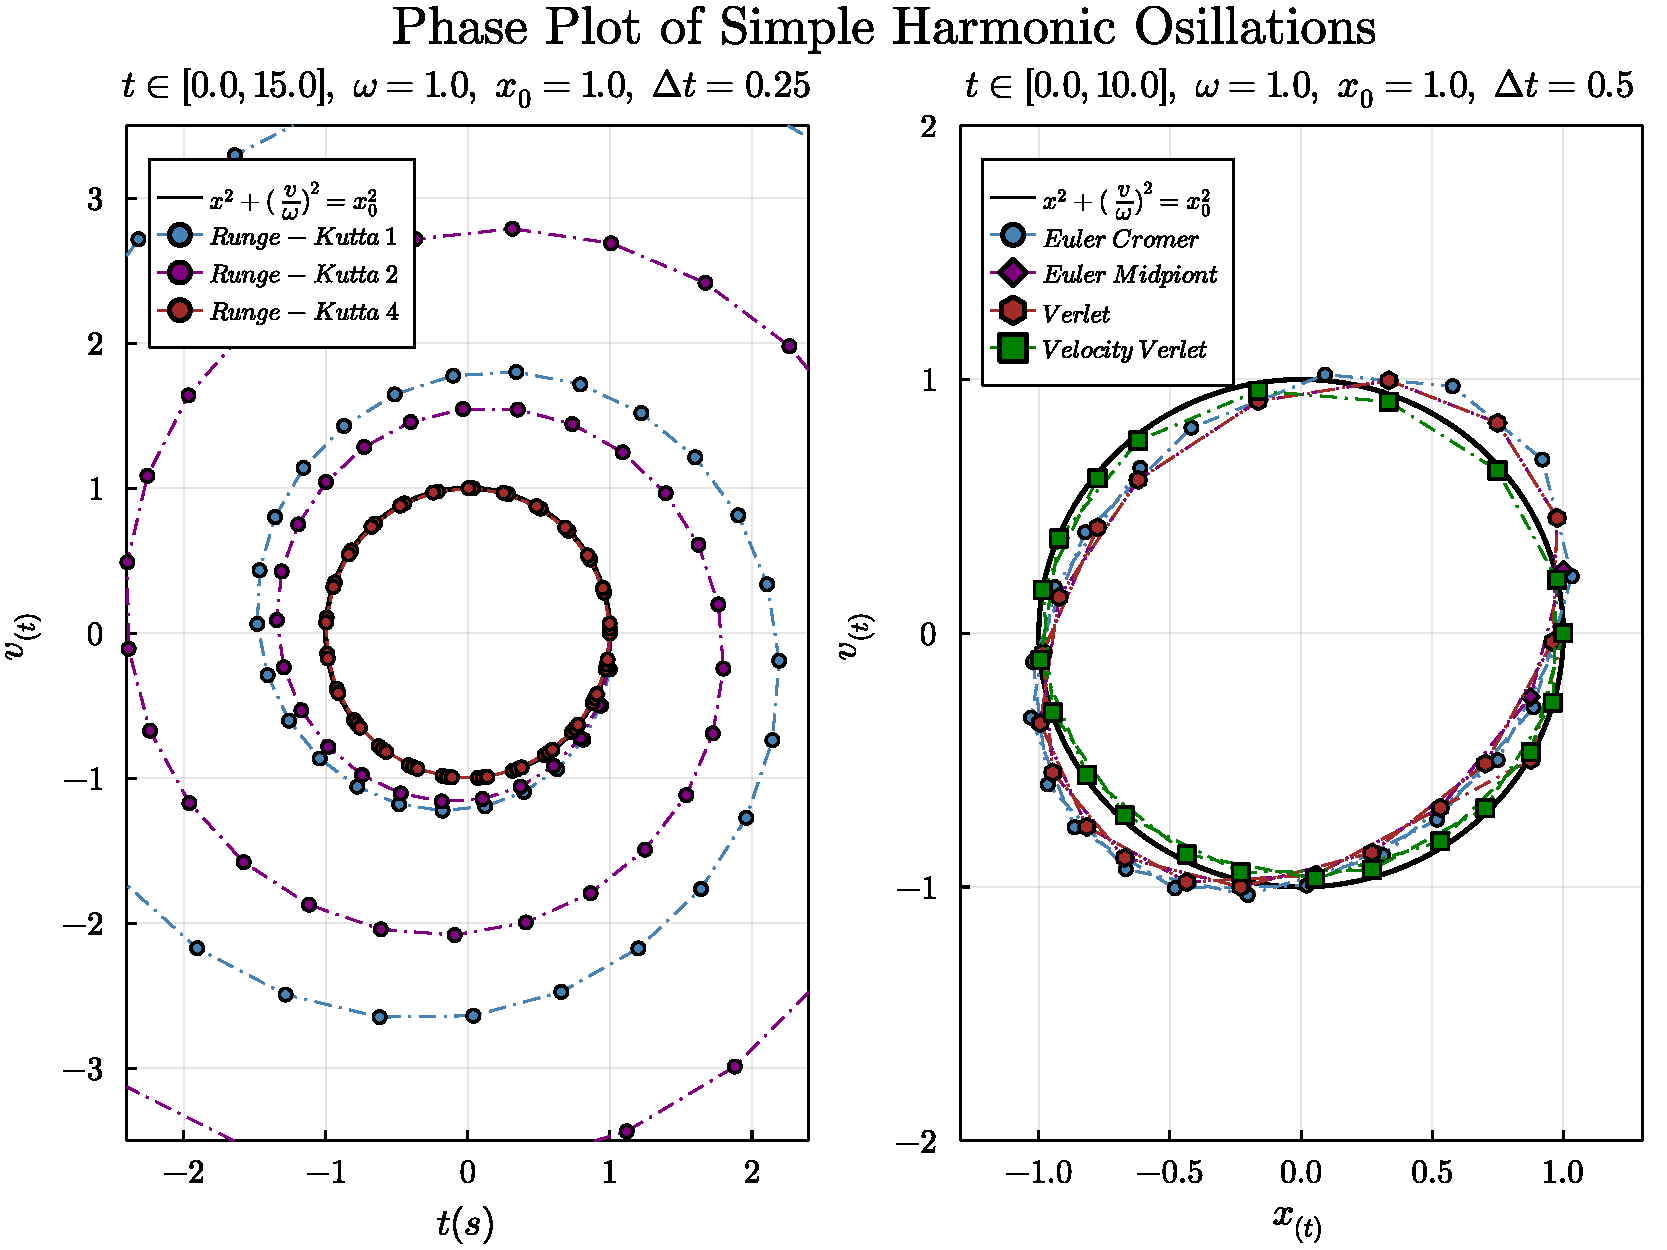
\includegraphics[scale = 0.3]{/Q2/Phase}
        \label{fig:2.2}
        \caption{Phase diagram of the oscillation.}
    \end{figure}

    In this section as well, we can see the energy conservation for each method and we can see that RK1 and RK2 methods do not follow that.

    \section{Logistic Map and bifurcations}
    \textbf{Basic description:}
    
    For this section, I wrote a code that creates a standard logistic map,
    finds bifurcation points, and exports their data.
    Then, find the wanted constant using exported data.

    \textbf{The results:}

    \begin{figure}[!htb]
        \centering
        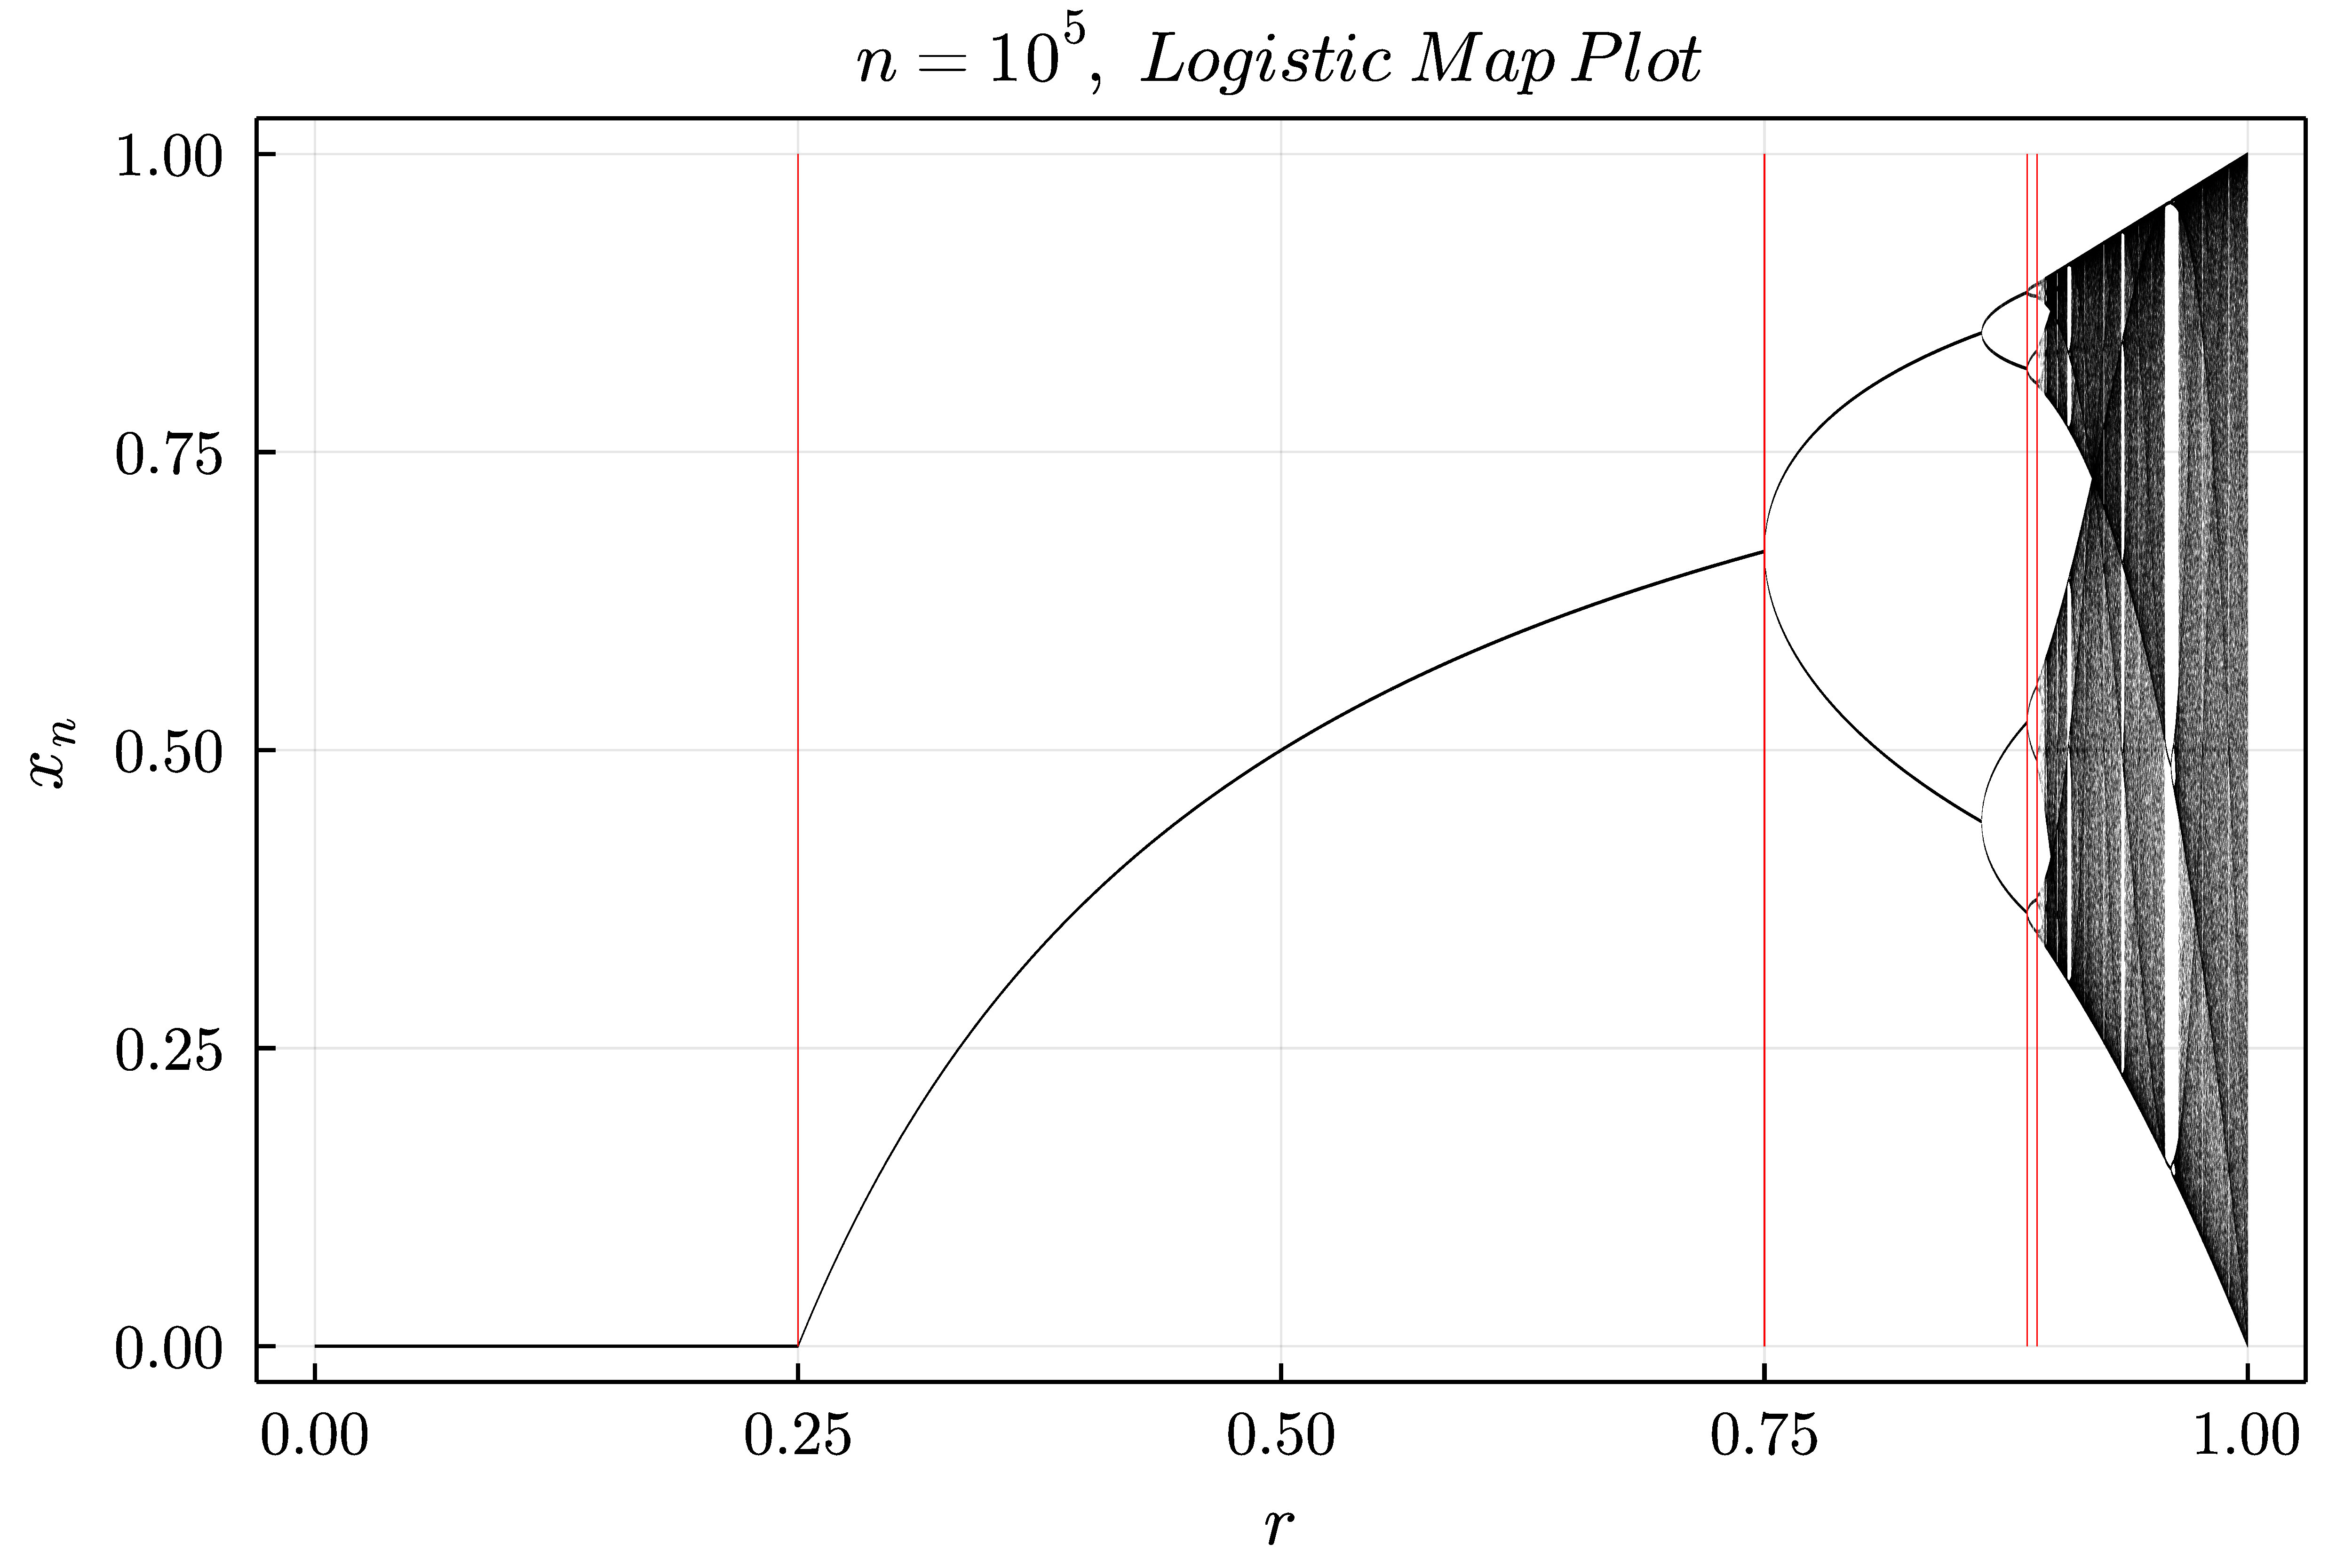
\includegraphics[scale = 0.4]{/Q3/logmap.jpg}
        \label{fig:3.1}
        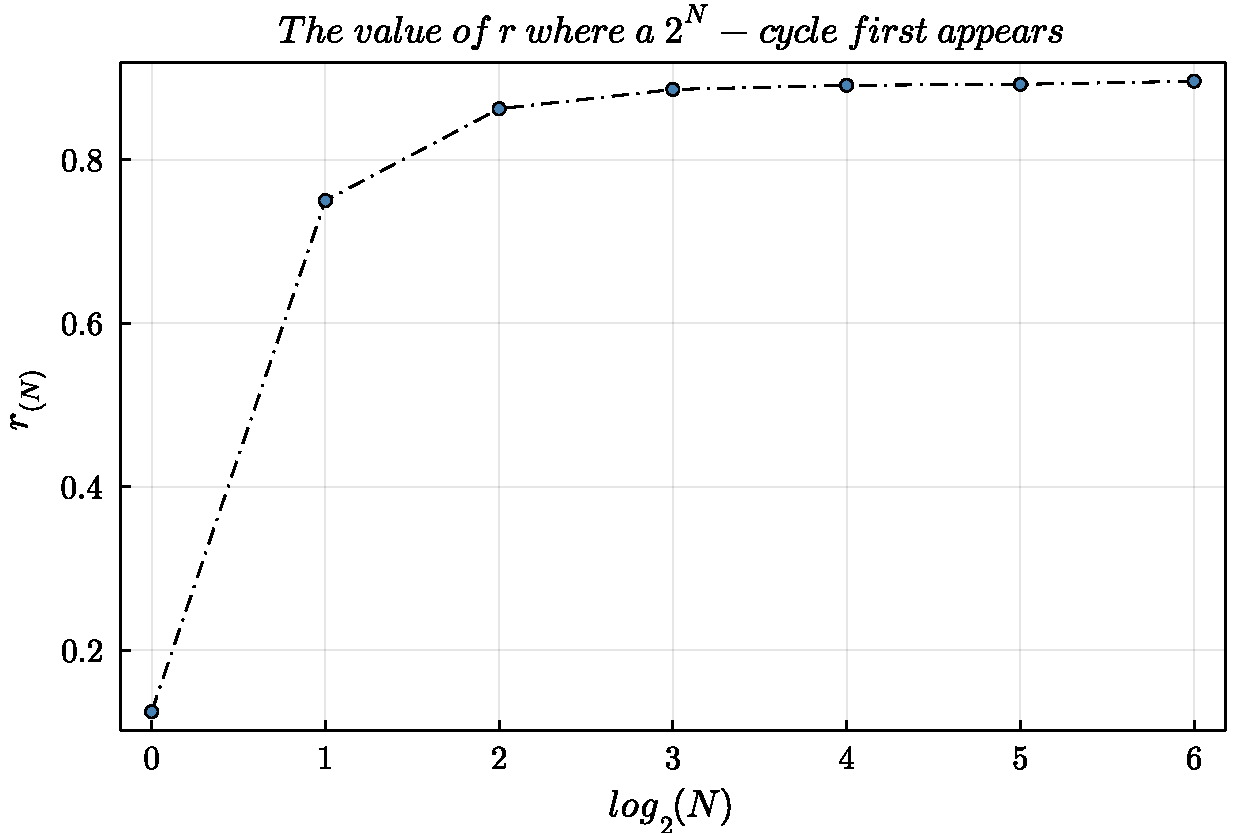
\includegraphics[scale = 0.4]{/Q3/R-N}
        \label{fig:3.2}
        \caption{Logistic Map diagram and bifurcation points.}
    \end{figure}

    Calculated constants:
    $$\delta = 4.6316,\ \alpha = 2.7143$$(take a look at the notebooks)

    \pagebreak

    \centering
    \textbf{The whole data I gathered is in \href{https://github.com/shahmari/ComputationalPhysics-Fall2021/tree/main/ProblemSet7/Data}{this link}}

    Thanks for watching :)
\end{document}